\section{Results and applications}
\label{sec:results}
A variety of noisy point clouds with sharp features are tested to evaluate the performance of our approach.
We also compare our method with some classic and state-of-the-art algorithms: PCA \cite{DBLP:conf/siggraph/HoppeDDMS92}, robust normal estimation (RNE) \cite{DBLP:journals/cg/LiSKCDJ10} and hough transform (HF) \cite{DBLP:journals/cgf/BoulchM12}.


To evaluate the estimation accuracy, the Root Mean Square measure with threshold ($RMS\_\tau $) \cite{DBLP:journals/cgf/BoulchM12} is used as follows:
\begin{equation}\label{eq:NEE}
RMS\_\tau = \sqrt{\frac{1}{|\mathcal{P}|}\sum_{p\in \mathcal{P}}(f(\widehat{n_{p,ref}n_{p,est}}))^{2}},
\end{equation}
where
$$f(\widehat{n_{p,ref}n_{p,est}})=\left \{
\begin{array}{rl}
    \widehat{n_{p,ref}n_{p,est}}, \quad & if\widehat{n_{p,ref}n_{p,est}}<\tau \\
    \pi /2,\quad & otherwise \\
\end{array}
\right. ,
$$
$n_{p,ref}$ is the reference normal at $p$ and $n_{p,est}$  is the
estimated one.
%
We take $\tau = 10$ degrees, as proposed by \cite{DBLP:journals/cgf/BoulchM12}. In the following, the points with the measure greater than $10$ degrees are considered as bad points.

%%%%%%%%%%%%%%%%%%%%%%%%%%%%%%%%%%%%%%%%%%%%%%%%%%%%%%%%%%%%%%%%%%%%%%%%%%%%%%%%%%%%%%%%%%%%%%%%%%%%%%%%%%%%
%%%%%%%%%%%%%%%%%%%%%%%%%%%%%%%%%%%%%%%%%%%%%%%%%%%%%%%%%%%%%%%%%%%%%%%%%%%%%%%%%%%%%%%%%%%%%%%%%%%%%%%%%%%%
The parameters $S$, $S^{*}$, $K$ and $r$ of our algorithm are chosen as $S=70$, $S^{*}=120$, $K=30$ and $r=10$ for all models in this section.
%
We use the same neighborhood size $S^{*}$ for all the three methods.
All other parameters, if any, are set to default.
%
We evaluate the estimation accuracy on the data with synthetic noise: a centered Gaussian noise with deviation defined as a percentage of average distance between points.
%We evaluate precision and speed on data with artificial noise: a centered Gaussian noise with deviation defined as a percentage of the diagonal of the axis-aligned bounding box.

\subsection{Comparisons with other methods}

\textbf{Sharp features with shallow angles.} In \fig~\ref{fig:octahedron_03_result}, we compare the normal estimation results of the Octahedron model. It contains sharp features generated by two intersection planes with shallow angles. Normals estimated by PCA are overly smoothed on/near sharp features. Those of HF are also a bit smooth, since normals produced by triples sampled from different sides are likely to vote for the same bin when the angle is shallow.
%
The bottom row of \fig~\ref{fig:octahedron_03_result} demonstrates that our algorithm  preserves sharp features better. We can see that the number of bad points and $RMS\_\tau$ are both smaller from our method, as shown in the middle row of \fig~\ref{fig:octahedron_03_result} and \tab \ref{tab:Computational_Statistics}.

\begin{figure}
\begin{center}
    \begin{tabular}{c}
        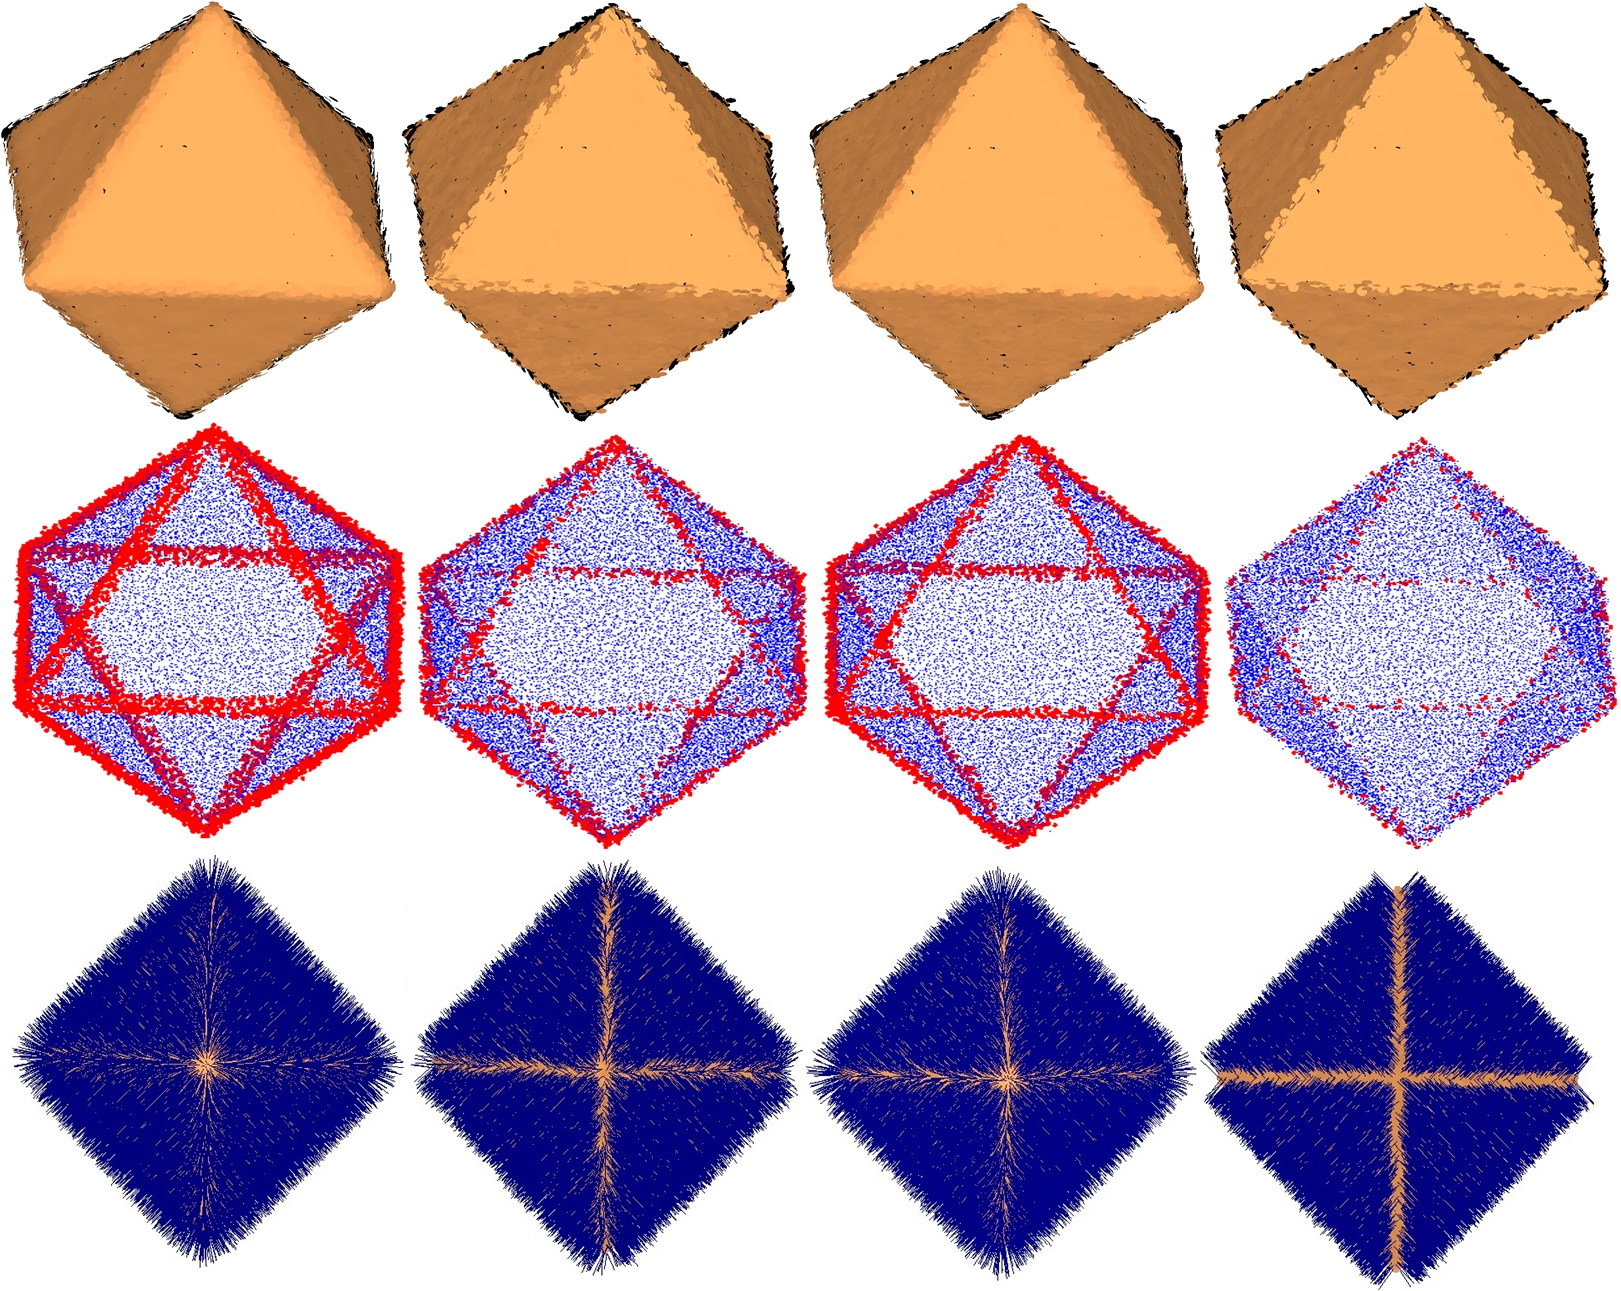
\includegraphics[width=1\linewidth]{oc}
    \end{tabular}
    \caption{Comparison for Octahedron model with $50\%$ noise.  From the top to bottom row are the results rendering using surfels, the visualization of bad points and top view of the generated normals, respectively. Left to right are the results of PCA, RNE, HF and our algorithm, respectively.\label{fig:octahedron_03_result}}
\end{center}
\end{figure}

\textbf{Neighborhood with multiple features.} The normal estimation results of Fandisk model are compared in \fig~\ref{fig:fandisk_01_result}.
%
The neighborhood of a point may contain multiple feature lines as the marked narrow-band regions in \fig~\ref{fig:fandisk_01_result}.
The complex neighborhood structure brings more challenges to the existing normal estimation methods.
%
As \fig~\ref{fig:fandisk_01_result} shown, PCA, RNE and HF generate more bad points around the narrow-band regions.
%
Our method utilizing the neighborhood's structure information does not have this flaw.
%
In addition, the bottom row of \fig~\ref{fig:fandisk_01_result} shows that our method preserves shape features comparatively better in presence of noise, while the others all blur sharp features.
%
%The bad points number and $RMS\_\tau$ listed in \tab \ref{tab:Computational_Statistics} provide further evidence to show the advantage of our method.



The bad point distributions of PCA, RNE, HF and our method are presented in \fig~\ref{fig:histogram} for the Octahedron and Fandisk models. We notice that the number of bad points from our method are much less than other methods in all normal deviation regions from 10 to 90 degree nearly.
%
For the Fandisk model, PCA obtains the smallest number of bad points with normal deviation between 80 to 90 degrees among all compared methods. It is because that the normals near sharp features by PCA are excessively smoothed and the largest deviations are almost 40 to 60 degrees.
%
%Based on the similar derivation, HF introduces a bit smoothness near sharp features and leads to less normal deviation between 70 to 90 degree.
%
The higher deviation between the above regions from RNE, HF and our method is mainly because that heavy noise makes the intersection of two planes becoming a ribbon from a line, where the points are supposed to have two directions.

\begin{figure*}[htbp]
\begin{center}
    \begin{tabular}{c}
        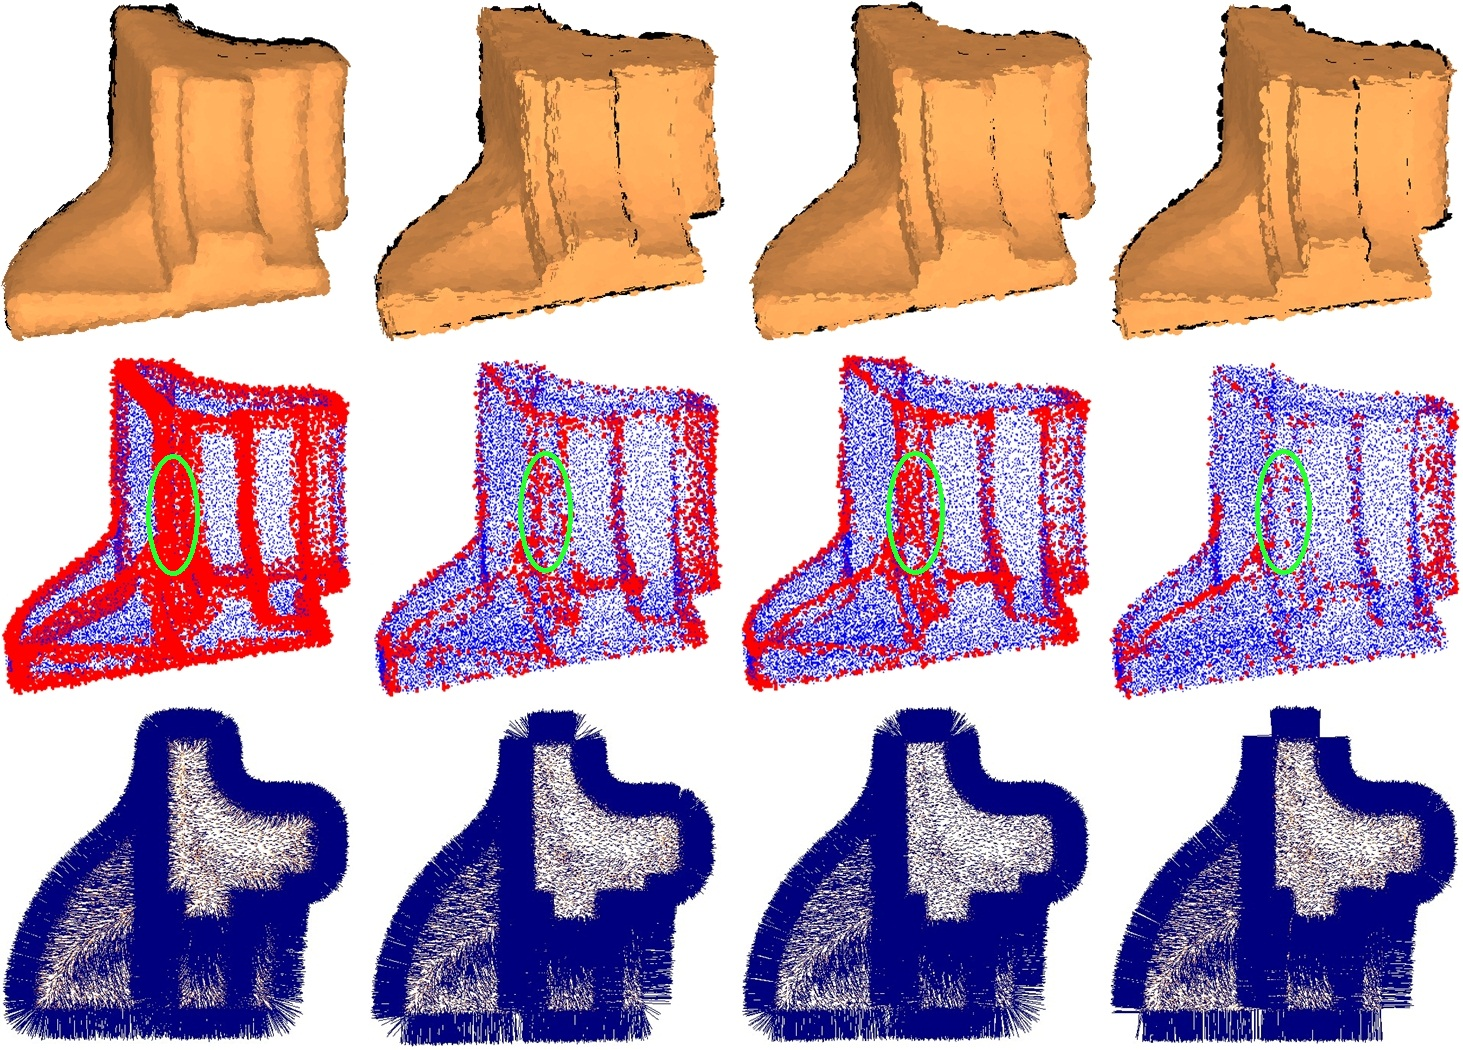
\includegraphics[width=0.8\linewidth]{fandisk_mark}\\
    \end{tabular}
    \caption{Comparison for Fandisk model with $50\%$ noise. From top to bottom row are the results rendering using surfels, the visualization of bad points and top view of the generated normals, respectively. Left to right are the results of PCA, RNE, HF and our algorithm, respectively.\label{fig:fandisk_01_result}}
\end{center}
\end{figure*}

\begin{figure*}[htbp]
\begin{center}
    \begin{tabular}{c c}
        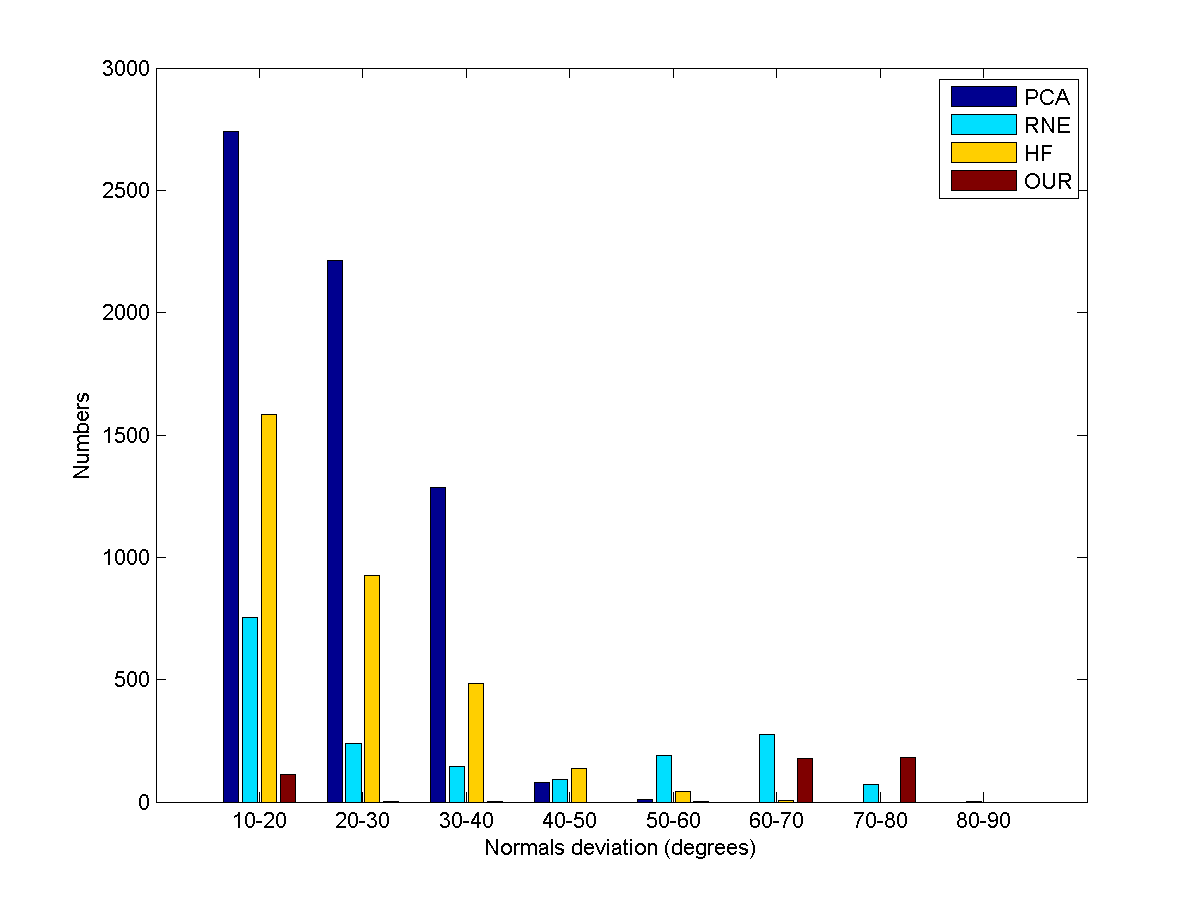
\includegraphics[width=0.5\linewidth]{octahedron_03_histogram} &
        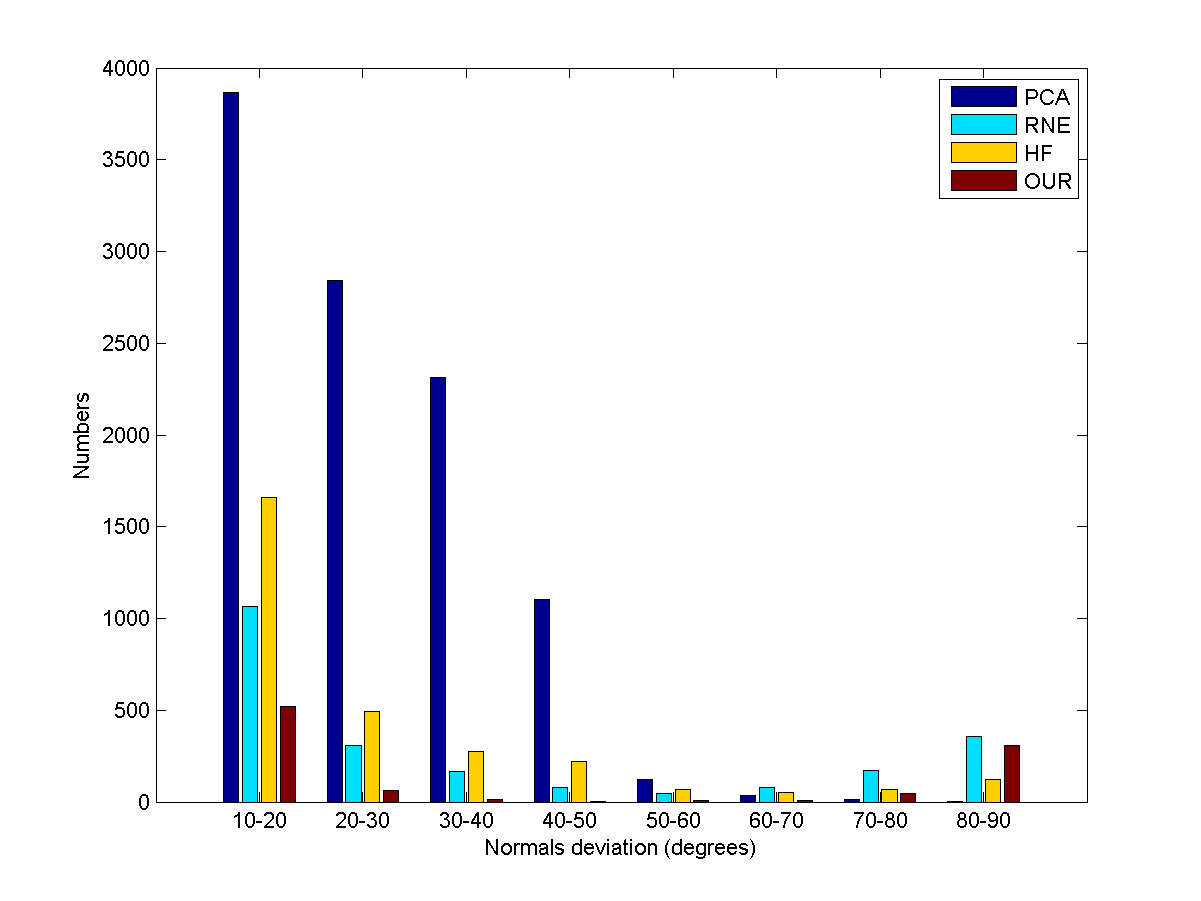
\includegraphics[width=0.5\linewidth]{fandisk_t1_histogram}
    \end{tabular}
    \caption{The histograms of the normal deviation on Octahedron model (left) and Fandisk model (right) shown in \fig \ref{fig:octahedron_03_result} and \fig \ref{fig:fandisk_01_result}, respectively.\label{fig:histogram}}
\end{center}
\end{figure*}

\textbf{Variational density near sharp features.}
Fig. \ref{fig:cube_02_result}  shows the normals estimated on a Cube sampled with face-specific
variations of density. PCA and RNE are severely affected by the non-uniform sampling. Since HF has designed a sampling strategy to deal with density variation, it performs better than PCA and RNE. However, there are still some errors near sharp features. Our method can effectively overcome the sampling anisotropy around sharp features.

%\begin{figure}[htbp]
%\begin{center}
%    \begin{tabular}{c}
%        \includegraphics[width=1\linewidth]{cube_t2_results}\\
%        \includegraphics[width=1\linewidth]{cube_t2_errs}
%    \end{tabular}
%    \caption{Results of Cube model with $50\%$ noise. Top is the estimated normals and bottom is the visualization of bad points. Left to right are the estimated results of PCA, RNE, HF and our algorithm, respectively.\label{fig:cube_02_result}}
%\end{center}
%\end{figure}
\begin{figure}[htbp]
\begin{center}
    \begin{tabular}{c c c c}
        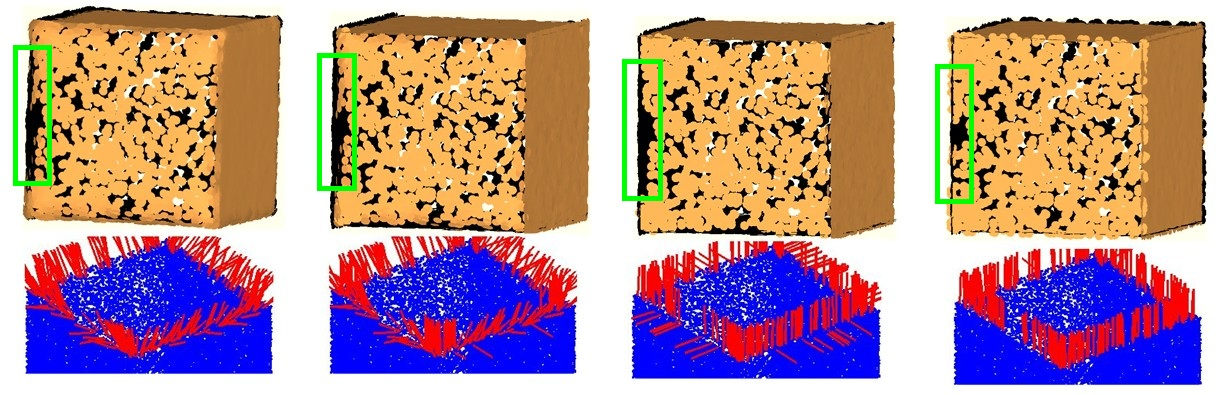
\includegraphics[width=1\linewidth]{cube}
    \end{tabular}
    \caption{Comparison for Cube model with $50\%$ noise. Density is uniform on each face; if density is 1 for the front face, then it is 5 for the upper face and 10 for the right face. The top row contains the results rendering using surfels, and the bottom row contains the top view of computed normals of the front face of the Cube model.  Left to right are the results of PCA, RNE, HF and our algorithm, respectively. \label{fig:cube_02_result}}
\end{center}
\end{figure}

\textbf{Computational statistics.}
To evaluate our method more precisely, models with different noise scales are computed, and $RMS\_\tau$ and the number of bad points are presented in Tab. \ref{tab:Computational_Statistics}. The statistics show that our method achieves the lowest $RMS\_\tau$ and NBP. More accurate normals are estimated under different noise scales.

\begin{table*}
\centering
\caption{\label{tab:Computational_Statistics}$RMS\_\tau$ and the number of bad points (NBP) on Fandisk, Octahedron  and Cube model with different noise scales.}
\begin{tabular}{|c|c|c|c|c|c|c|c|c|c|}
\hline
\multirow{2}{*}{Model} & \multirow{2}{*}{Noise scale} & \multicolumn{2}{|c}{PCA} & \multicolumn{2}{|c}{RNE} & \multicolumn{2}{|c}{HF} & \multicolumn{2}{|c|}{OUR} \\
\cline{3-10}
  & & $RMS\_\tau$ & NBP & $RMS\_\tau $ & NBP & $RMS\_\tau $ & NBP & $RMS\_\tau $ & NBP\\
\hline \hline
 Octahedron & $40\%$ & 0.7730 & 6338 & 0.3115 & 1005 & 0.4399 & 2034 & \textbf{0.1424} & \textbf{200} \\
 Octahedron & $50\%$ & 0.7722 & 6324 & 0.4123 & 1772 & 0.5496 & 3183 & \textbf{0.2174} & \textbf{478} \\
 Octahedron & $60\%$ & 0.7773 & 6406 & 0.4910 & 2518 & 0.6161 & 4002& \textbf{0.2986} & \textbf{914} \\
 Fandisk & $40\%$ & 0.9874 & 10206 & 0.3708 & 1469 & 0.4022 & 1668 & \textbf{0.2601} & \textbf{688} \\
 Fandisk & $50\%$ & 0.9921 & 10303 & 0.4694 & 2272 & 0.5341 & 2957 & \textbf{0.3088} & \textbf{970} \\
 Fandisk & $60\%$ & 1.0010 & 10487 & 0.5578 & 3214 & 0.6568 & 4485 & \textbf{0.3809} & \textbf{1483} \\
 Cube & $40\%$ & 0.5889 & 4510 & 0.2606 & 879 & 0.1043 & 135 & \textbf{0.0667} & \textbf{51} \\
 Cube & $50\%$ & 0.5865 & 4473 & 0.2537 & 829 & 0.1063 & 138 & \textbf{0.0674} & \textbf{50} \\
 Cube & $60\%$ & 0.5864 & 4471 & 0.2577 & 851 & 0.1147 & 159 & \textbf{0.0851} & \textbf{82} \\
\hline
\end{tabular}
\end{table*}

\subsection{More results for raw scans of real objects}
\label{sec:moreResults}
We also apply our method to real scanned point clouds, see~\fig~\ref{fig:realObjects} and~\fig~\ref{fig:shutter}, in which the typical imperfections, such as noise, outliers and non-uniform distribution are ubiquitous.
%-demonstrate the efficacy of our algorithm.
Although the edges of these models are corrupted with noise, especially for the Genus2 and Box models in ~\fig~\ref{fig:realObjects}, our algorithm recovers them faithfully.
%-
The Genus2 model also contains close-by surface sheets in the marked regions. The normal estimation approaches based on distance, such as PCA and its variants, tend to be affected greatly, while our structure based method not.
%-
Both the Armadillon and Taichi models are non-uniform sampled. The Taichi model has complex structures in the marked region of~\fig~\ref{fig:realObjects}. Our algorithm preserves the sharp feature well even in such complicated case.
%-
Tiny structures challenge normal estimation. The Shutter in~\fig~\ref{fig:shutter} contains many such tiny structures. When some of them are sampled adequately as the marked region, faithful normals are estimated by our method and the tiny structures can be visualized clearer.

\begin{figure*}
\begin{center}
    \begin{tabular}{c}
        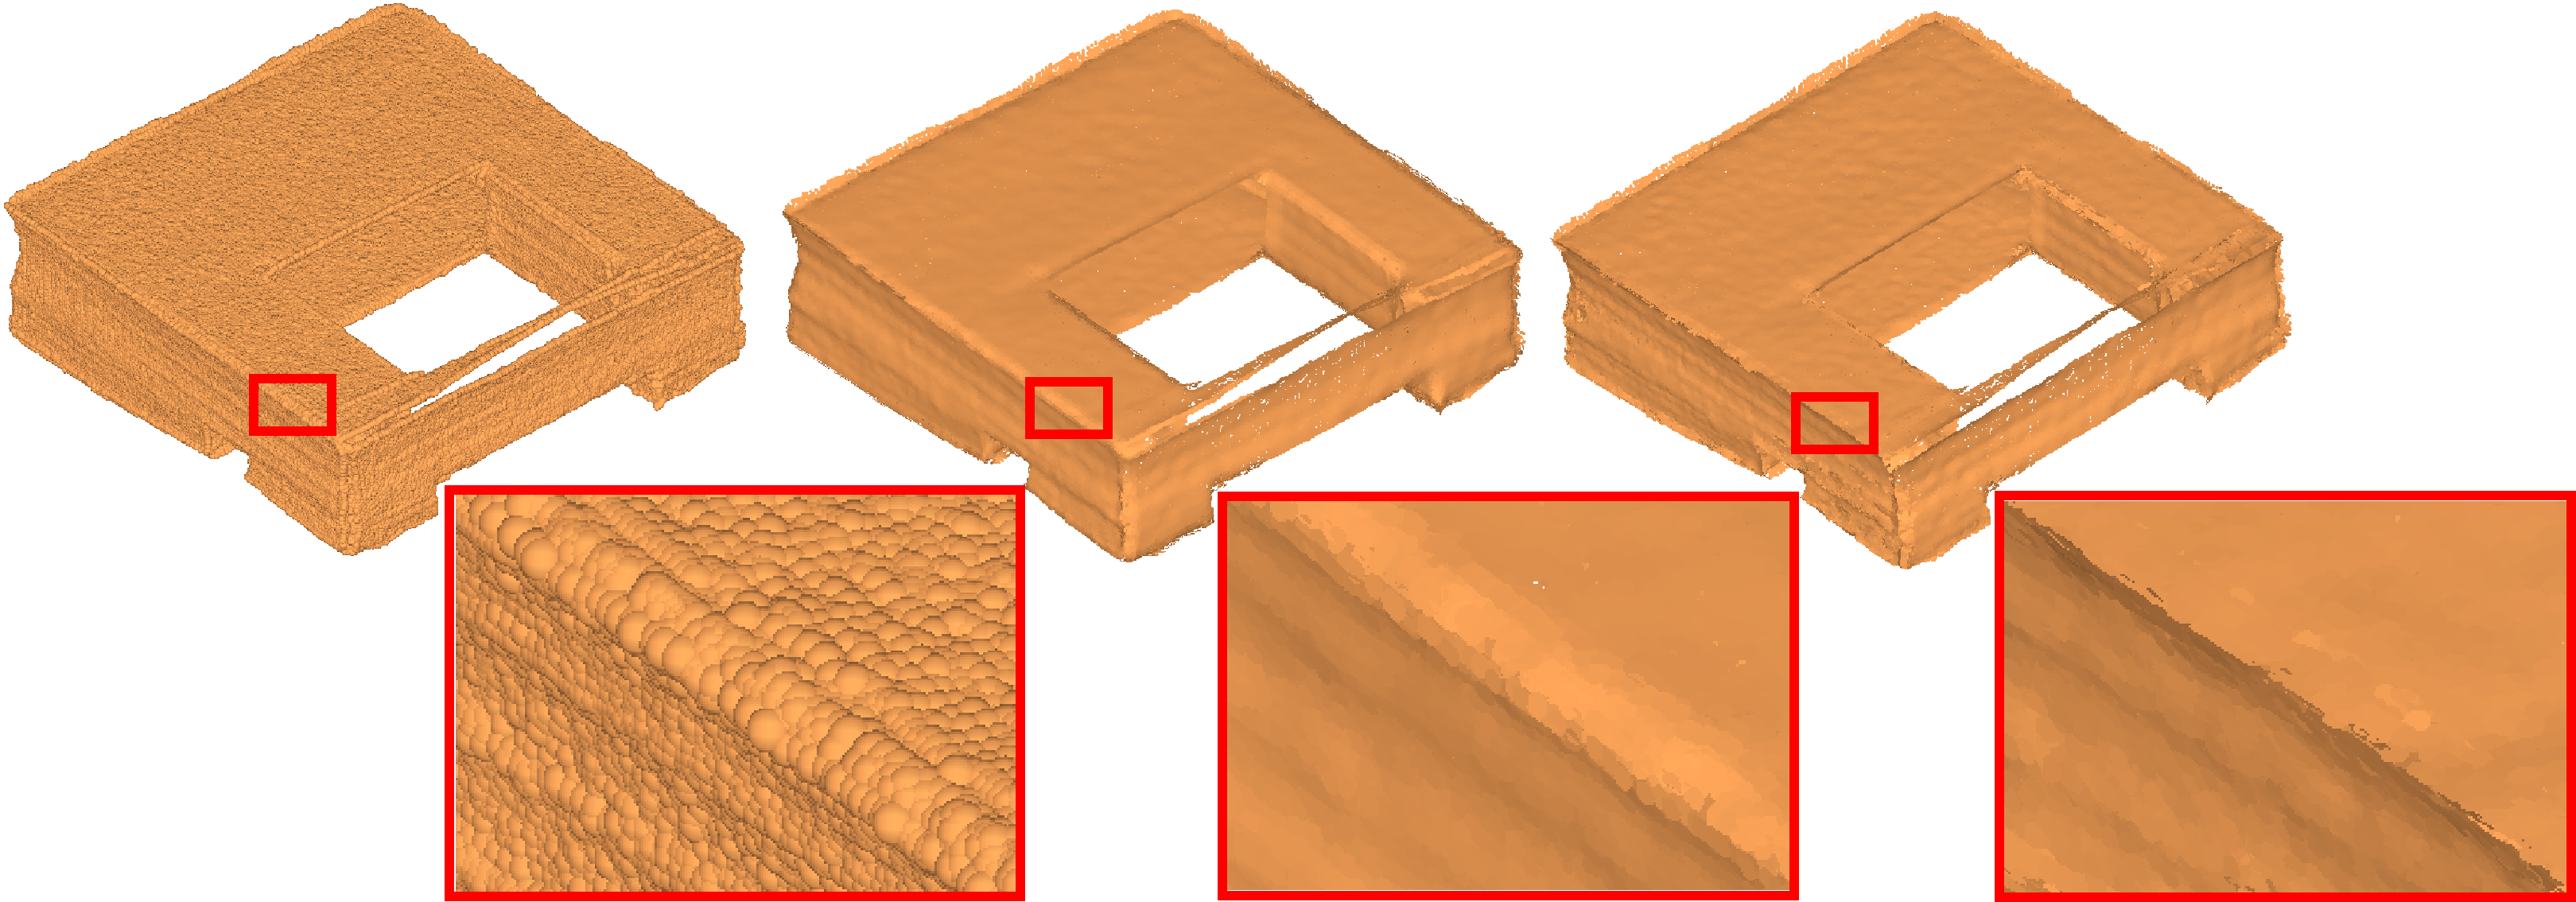
\includegraphics[width=0.8\linewidth]{box}\\
        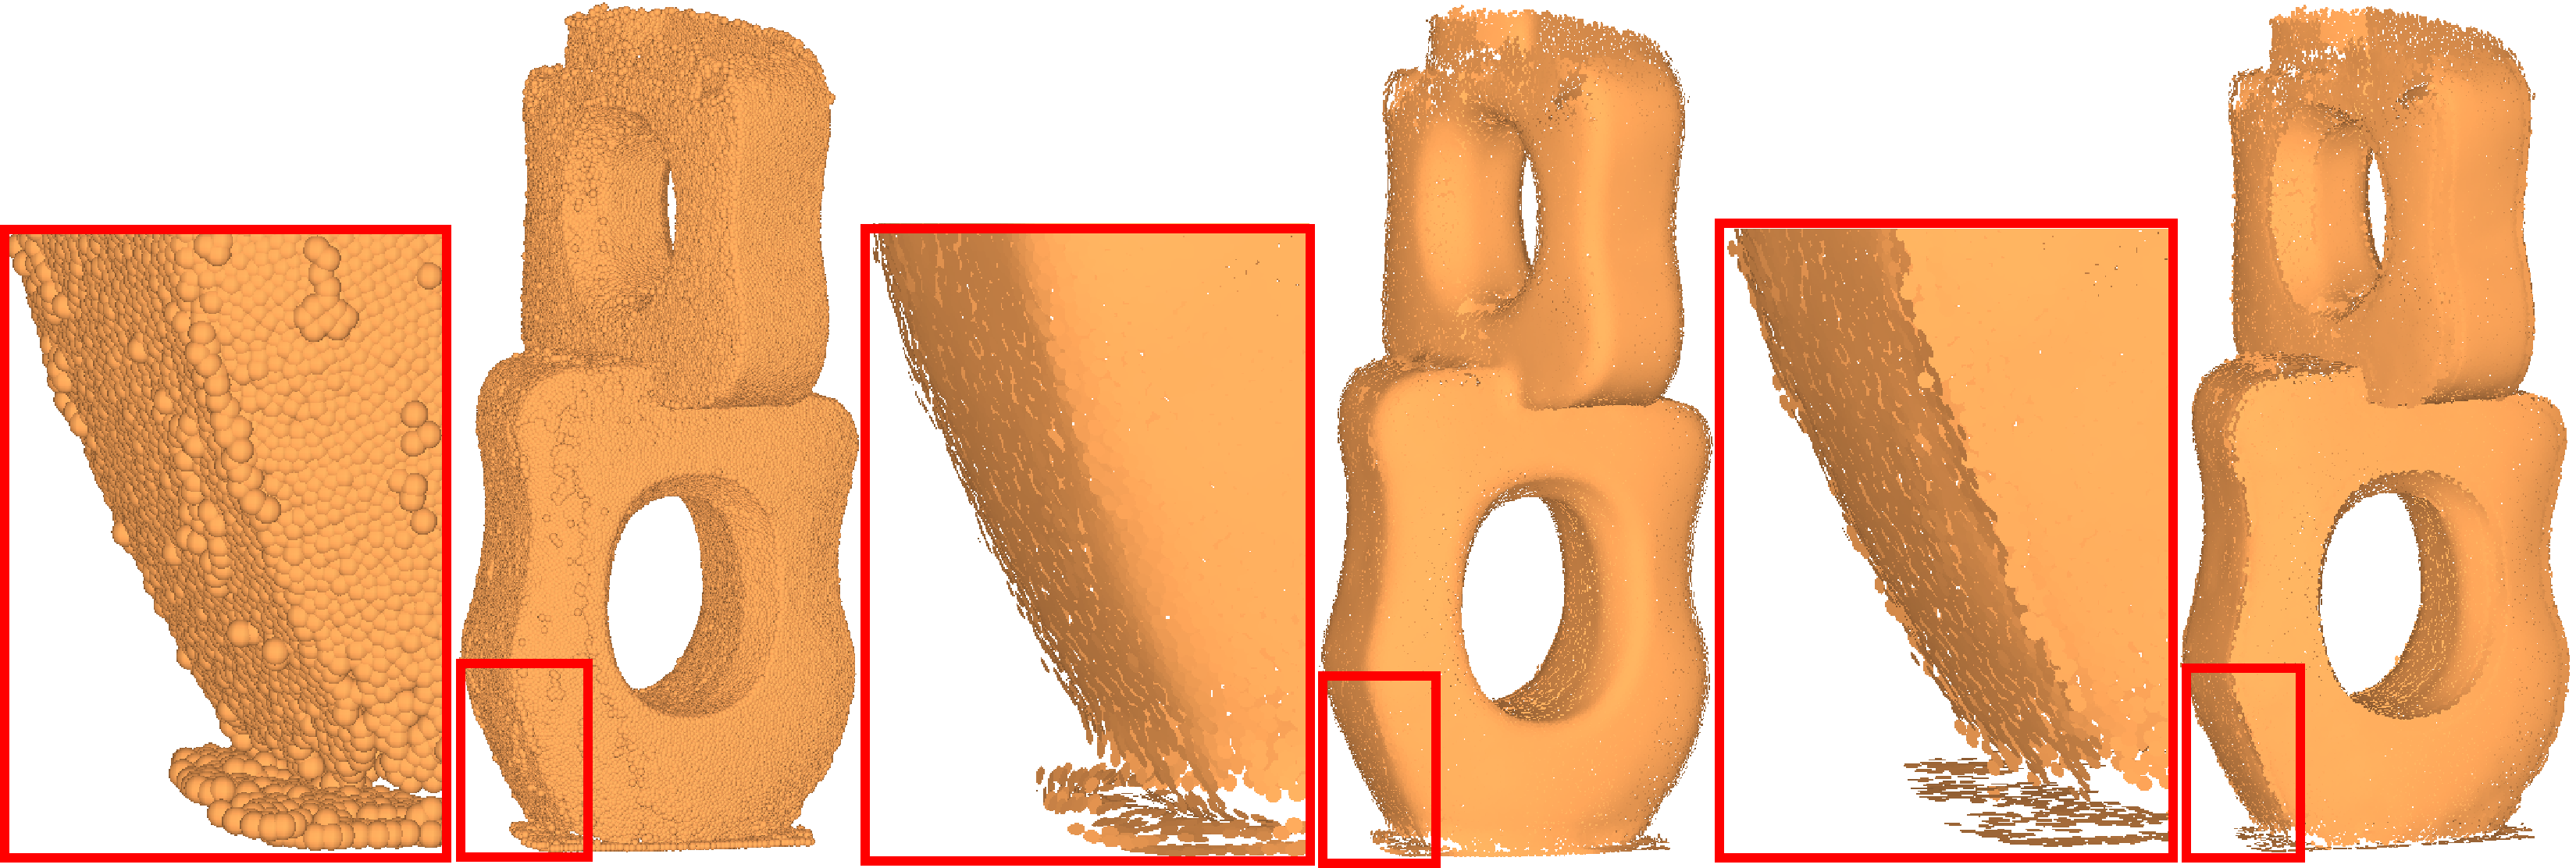
\includegraphics[width=0.8\linewidth]{geners1}\\
        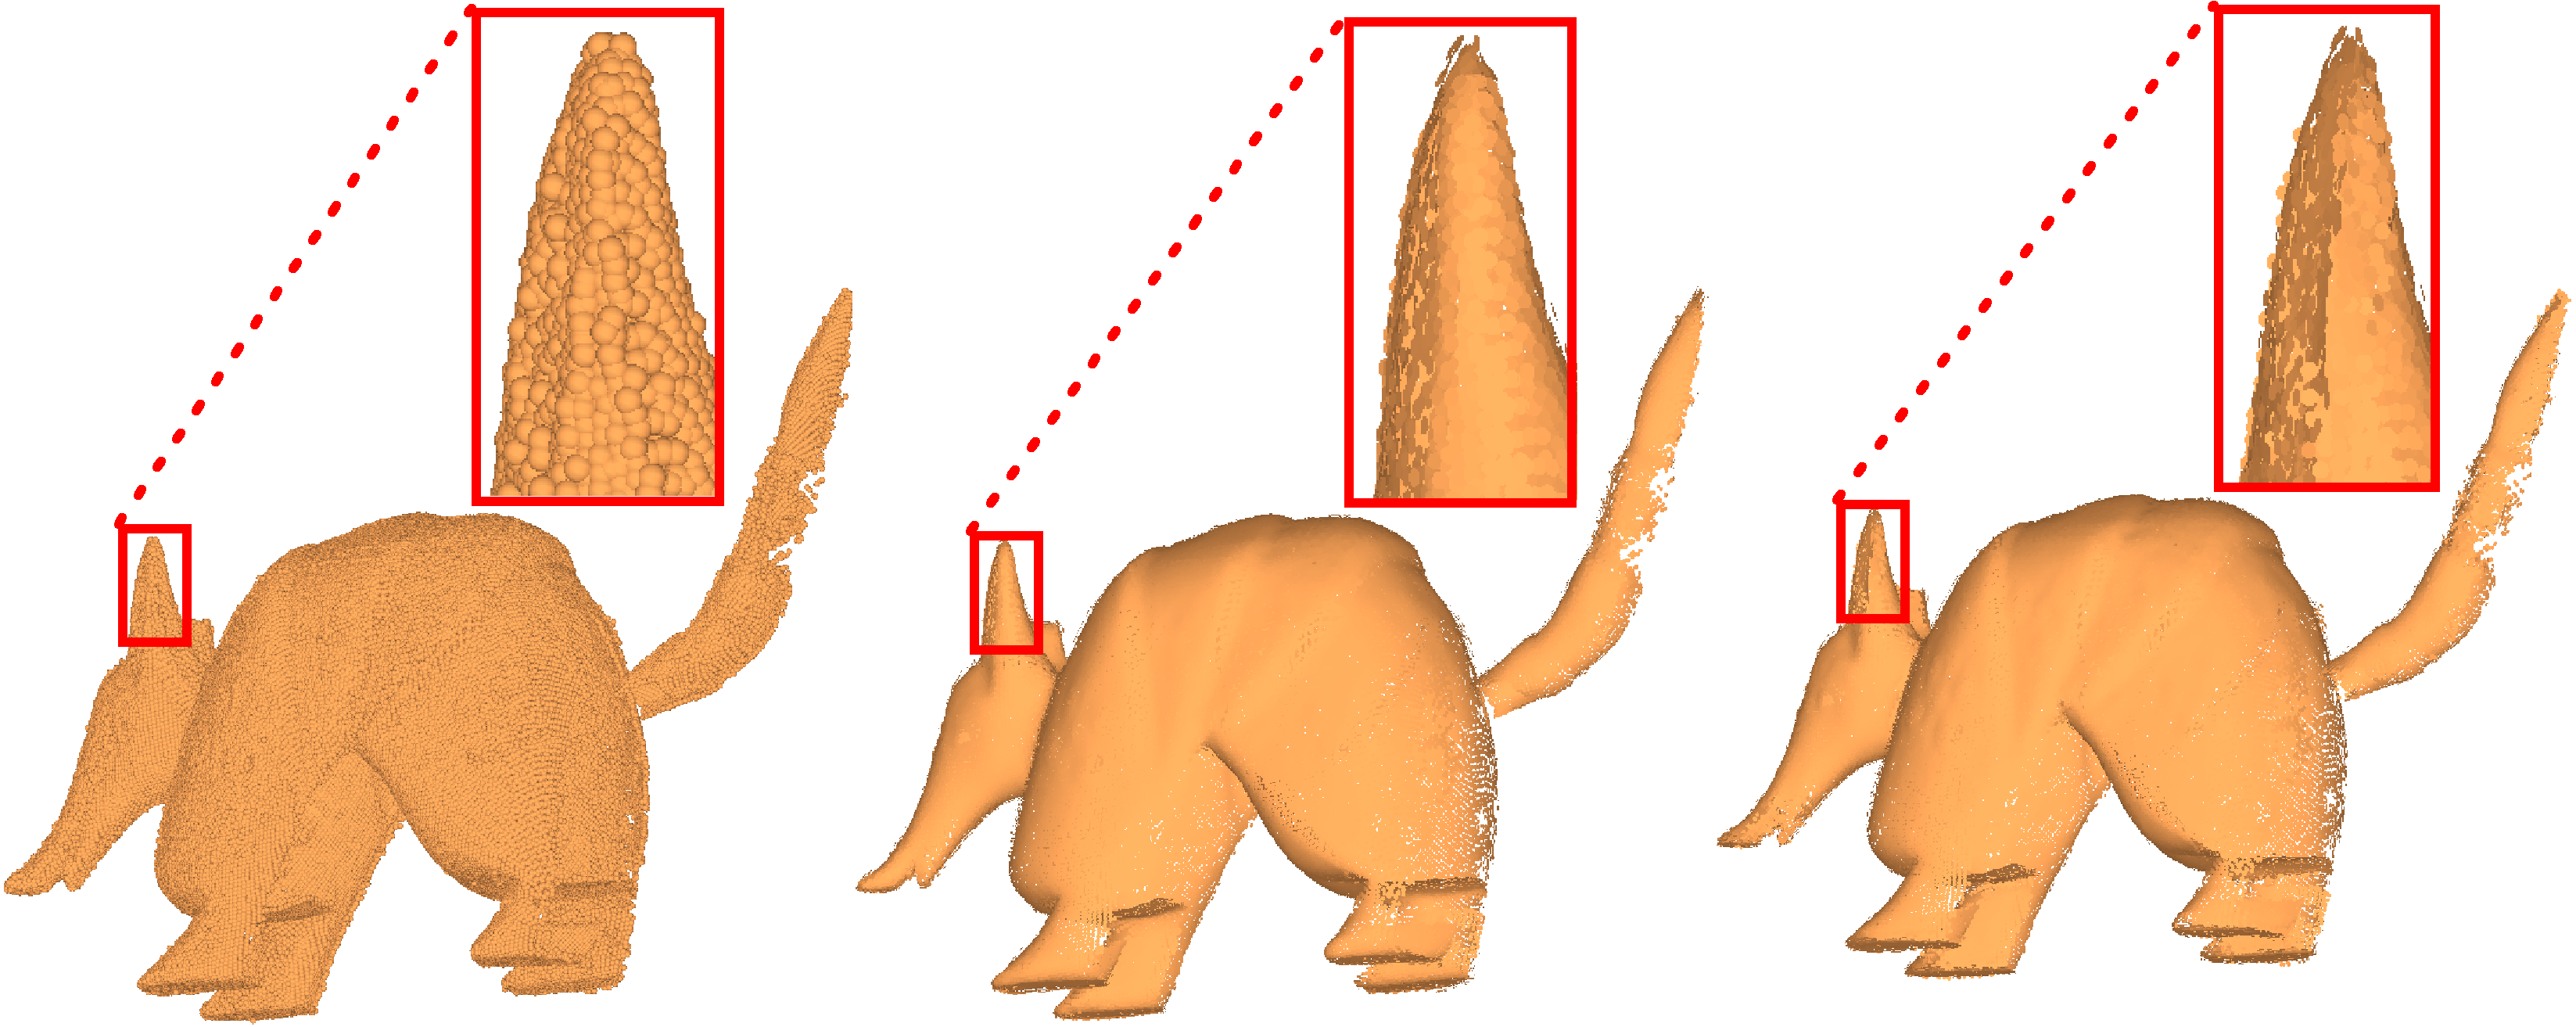
\includegraphics[width=0.8\linewidth]{armadillon}\\
        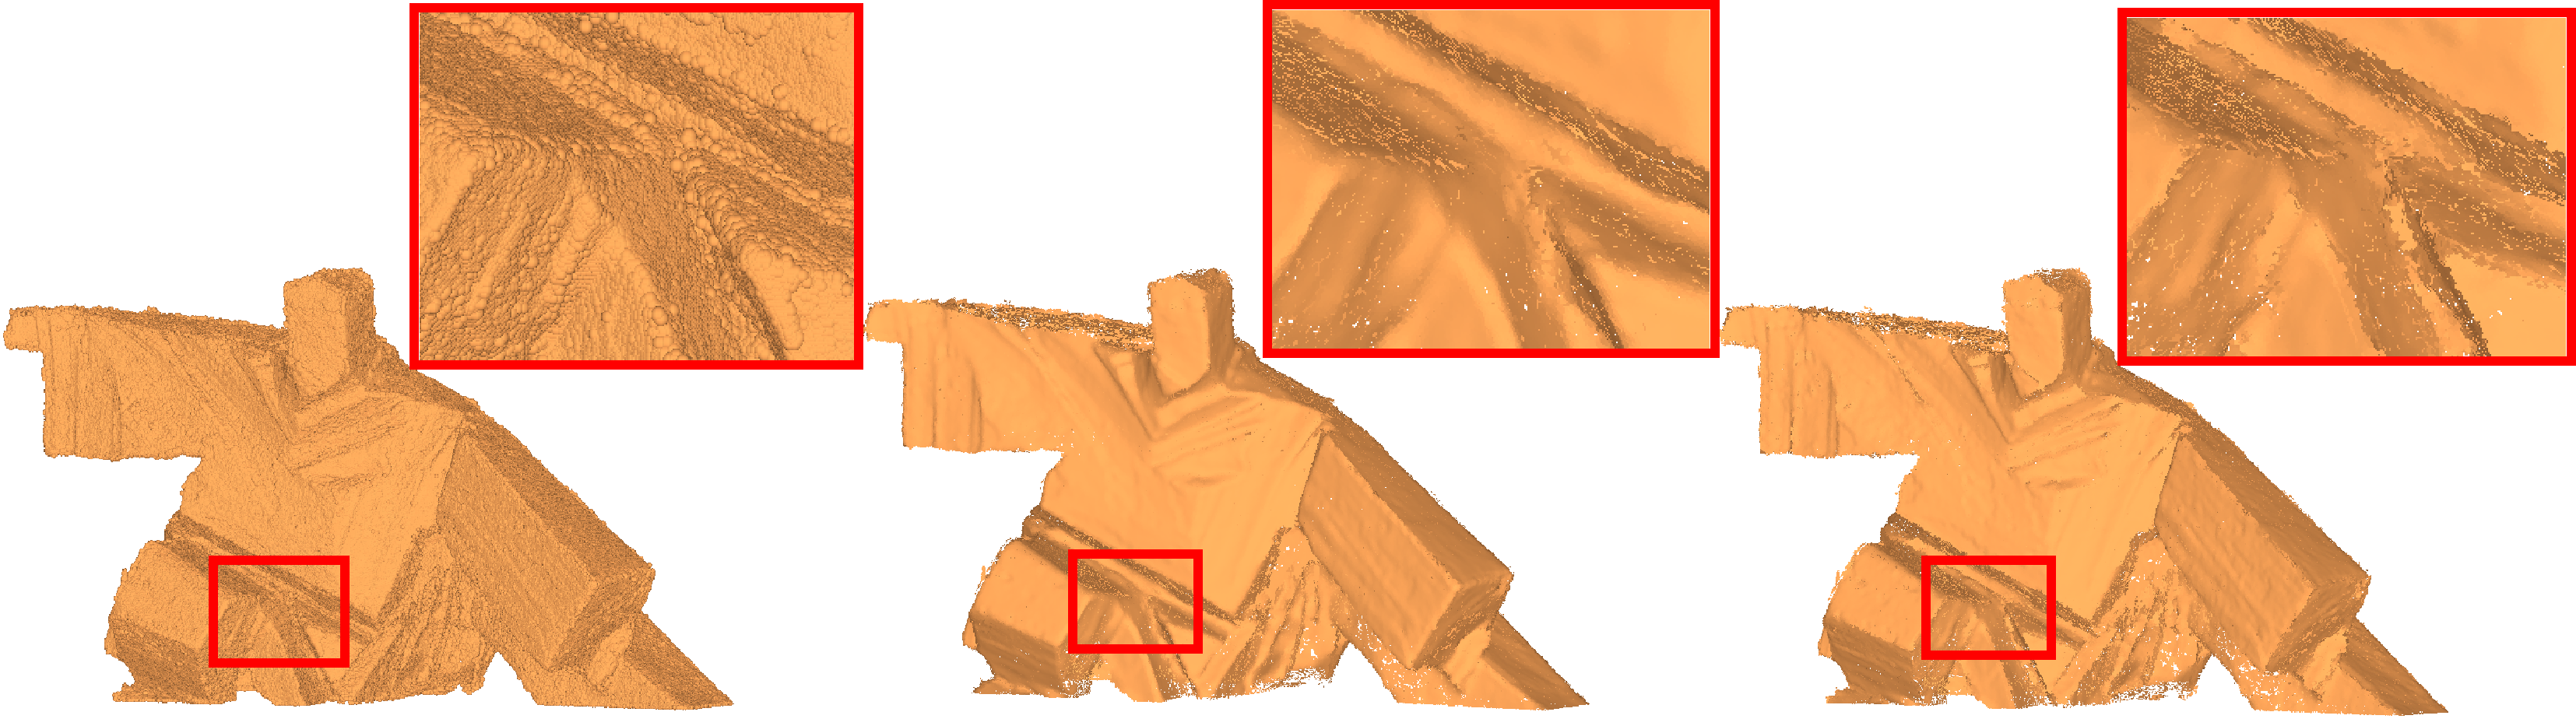
\includegraphics[width=0.8\linewidth]{taichi}\\
    \end{tabular}
    \caption{Normal estimation for raw scans of real objects: Box (222.5k points), Genus2 (50k points), Armadillon (99.4k points) and Taichi (537.6k points). Left to right are the input model, the results of PCA and our algorithm, respectively.\label{fig:realObjects}}
\end{center}
\end{figure*}

\begin{figure}
\begin{center}
    \begin{tabular}{c c }
        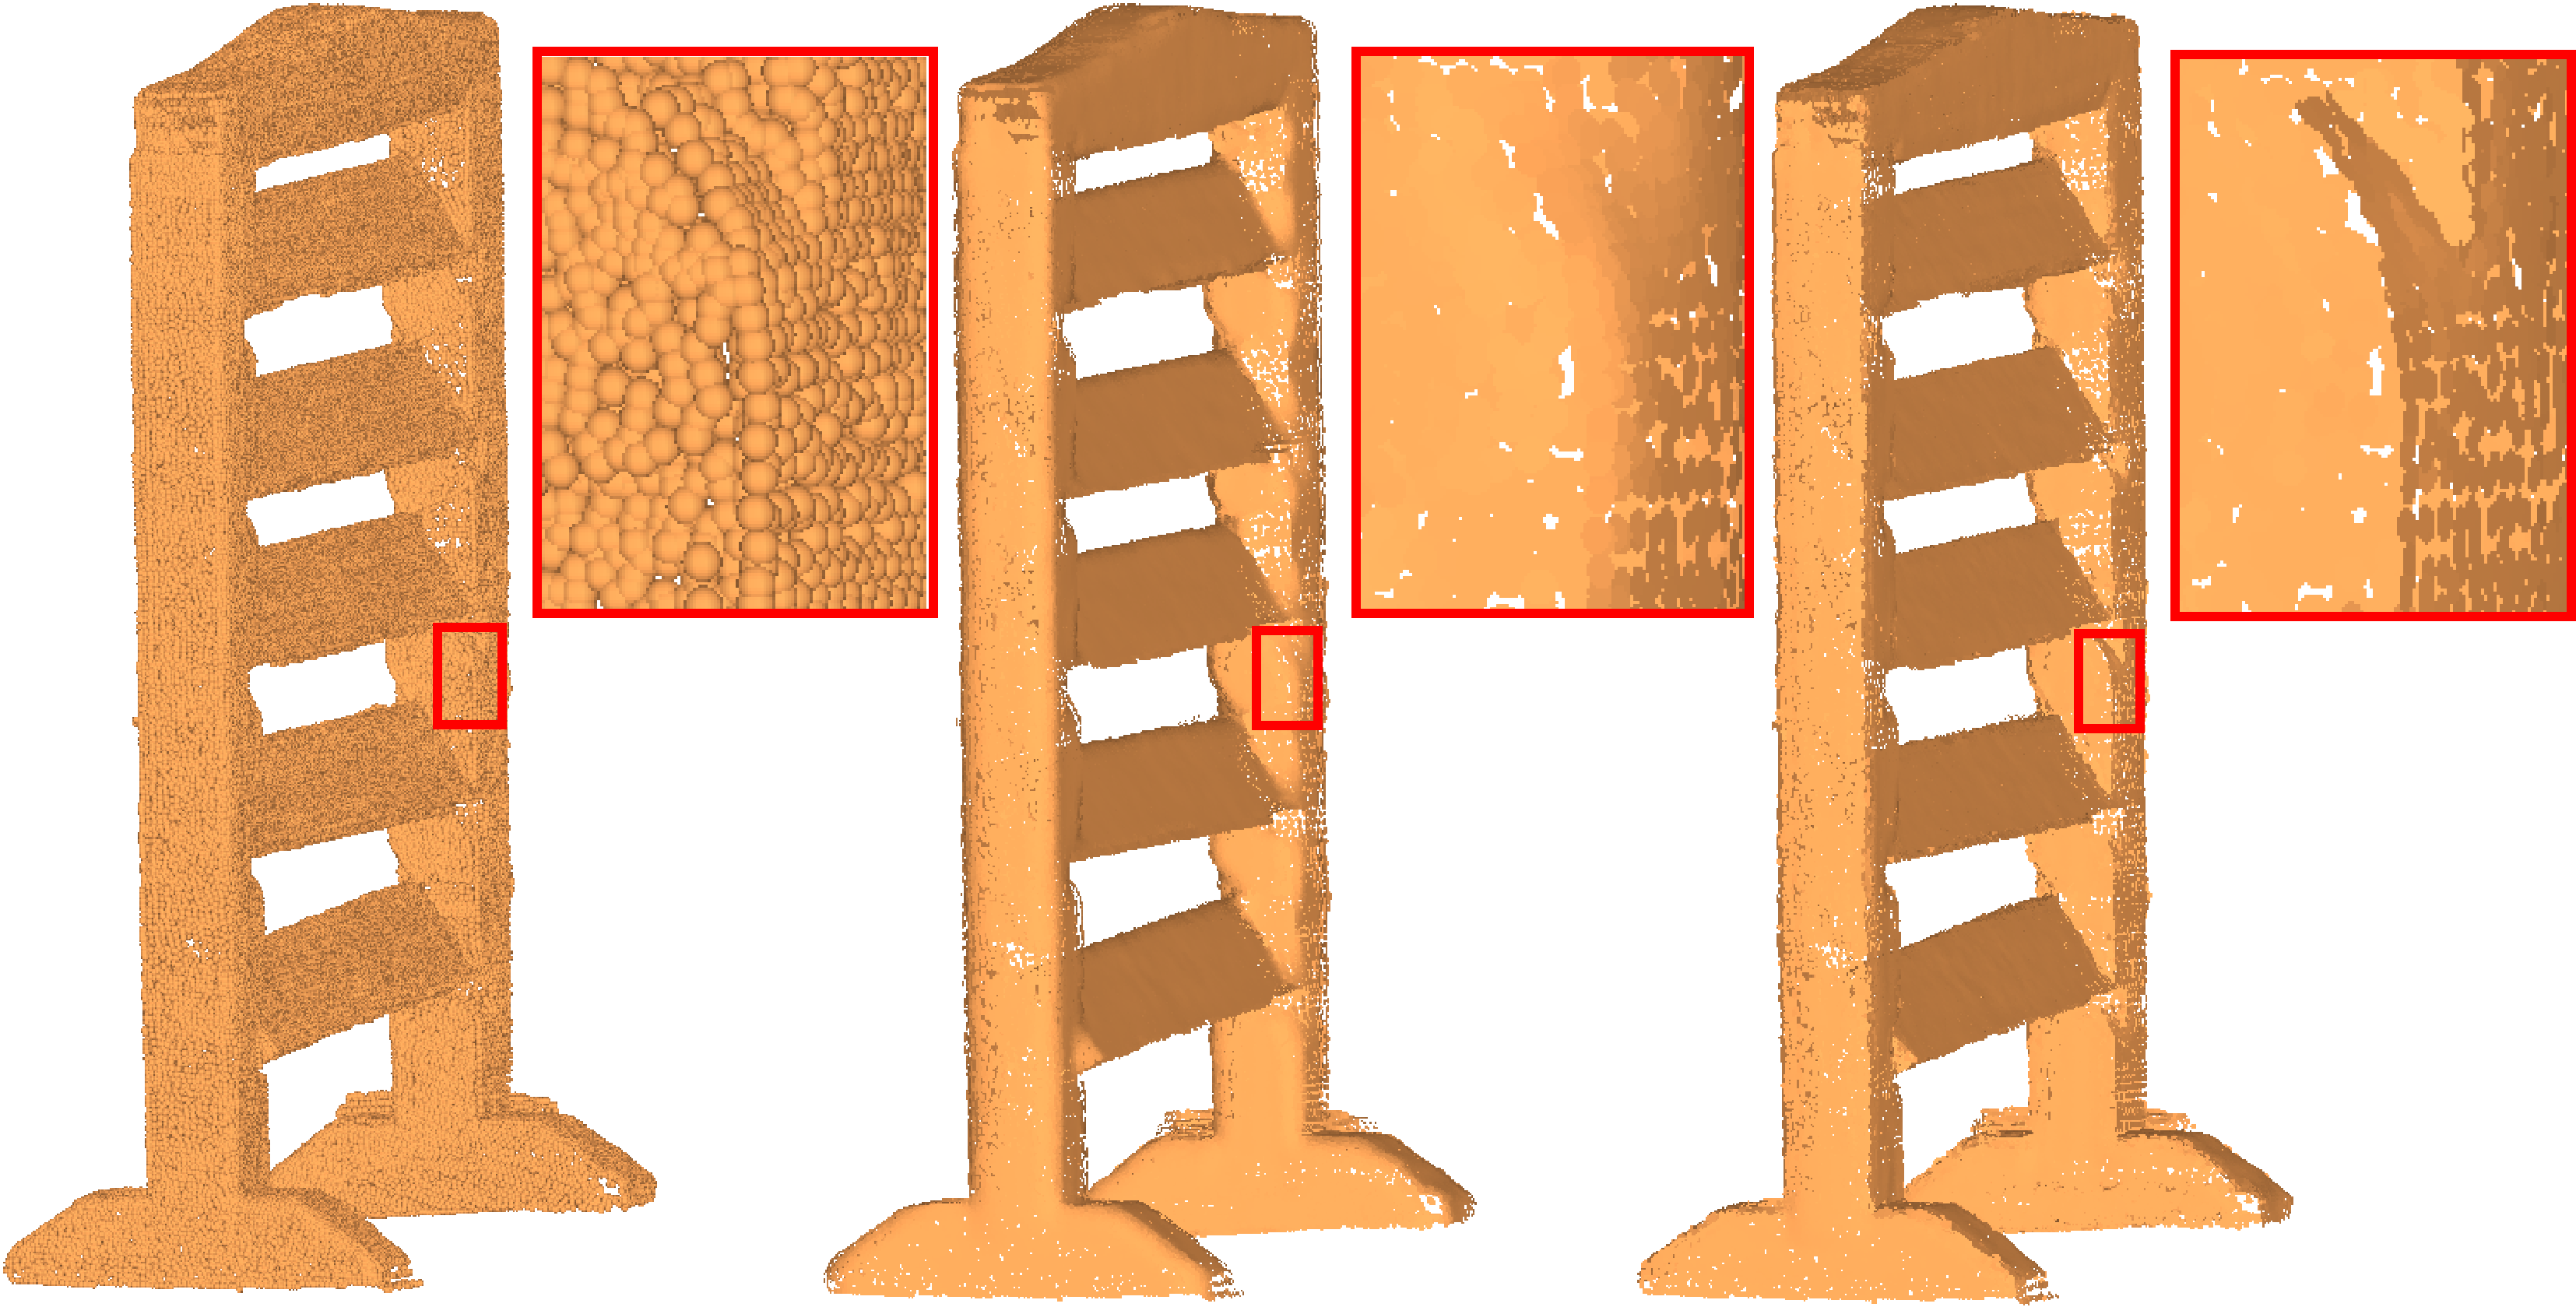
\includegraphics[width=1\linewidth]{shutter}
    \end{tabular}
    \caption{Normal estimation for the Shutter model. Left to right are the input raw scan model with 291.2k points, the results of PCA and our algorithm, respectively. \label{fig:shutter}}
\end{center}
\end{figure}
%Box (222.5k points <222481>), Genus2 (50k points <50050>), Armadillon (99.4k points <99416>) and Taichi (537.6k points <537564>), Shutter (291.2k points <291219>).
%\begin{figure*}
%\begin{center}
%    \begin{tabular}{c c }
%        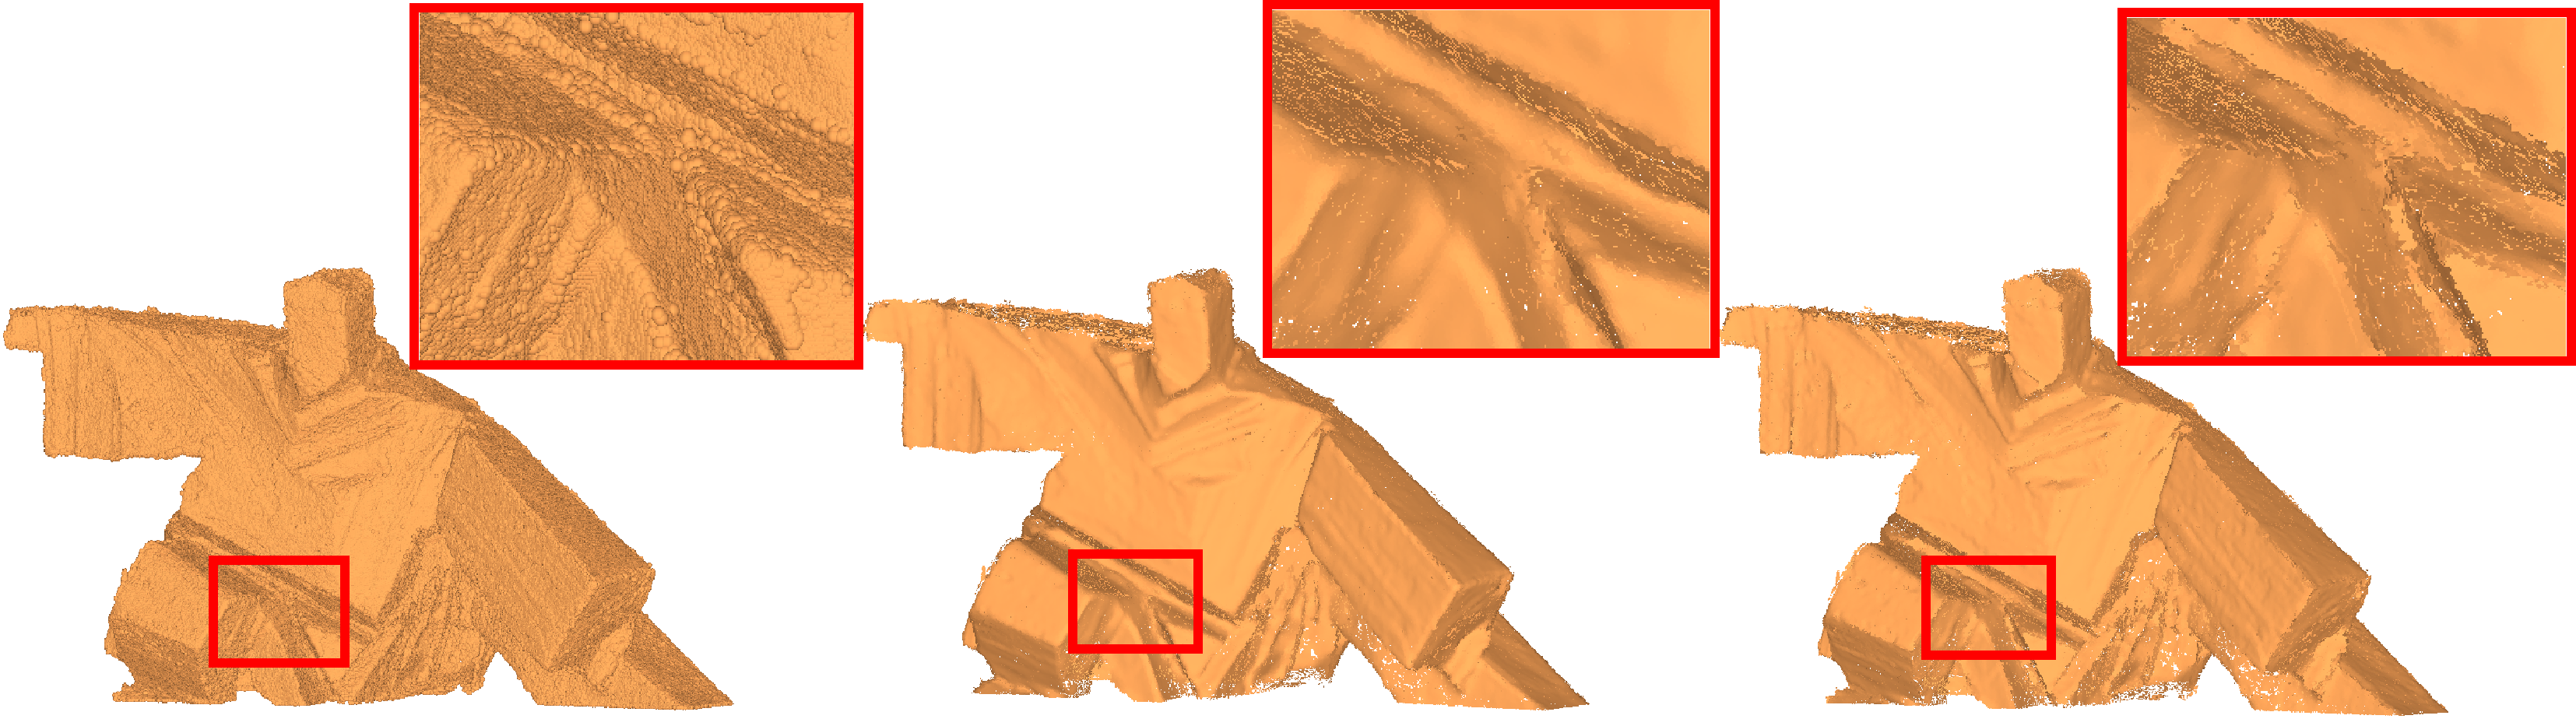
\includegraphics[width=1\linewidth]{taichi}
%    \end{tabular}
%    \caption{{\color{red}Normal estimation results for Taichi by using PCA and our algorithm. Left to
%     right are the raw scan, the results of PCA and our algorithm, respectively.}\label{fig:taichi}}
%\end{center}
%\end{figure*}
%\begin{figure*}
%\begin{center}
%    \begin{tabular}{c c }
%        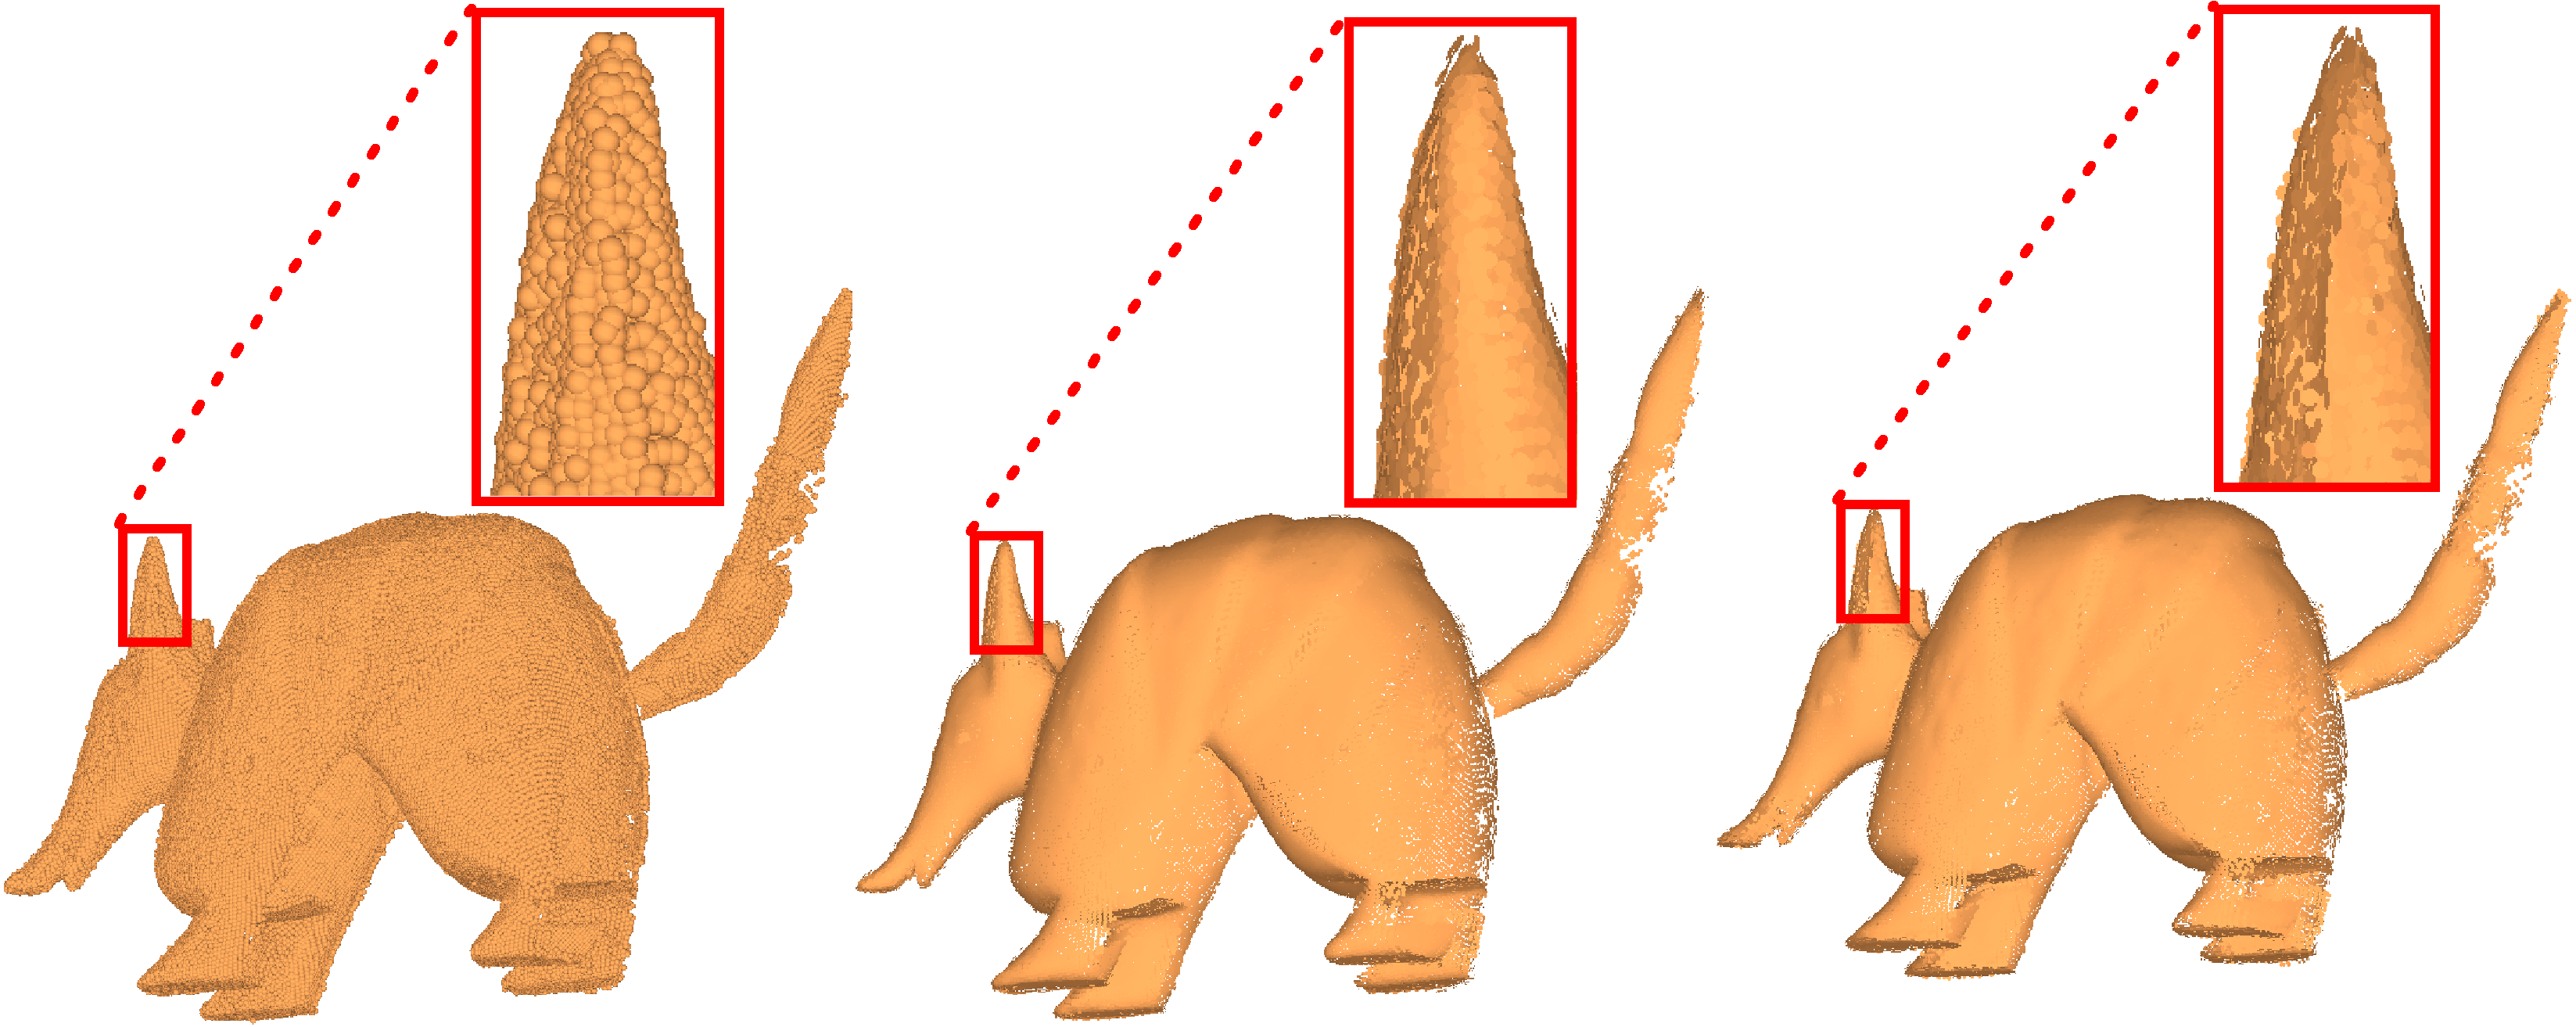
\includegraphics[width=1.0\linewidth]{armadillon}
%    \end{tabular}
%    \caption{{\color{red}Normal estimation results for Armadillon by using PCA and our algorithm. Left to
%     right are the raw scan, the results of PCA and our algorithm, respectively.}\label{fig:armadillo}}
%\end{center}
%\end{figure*}
%\begin{figure*}
%\begin{center}
%    \begin{tabular}{c c }
%        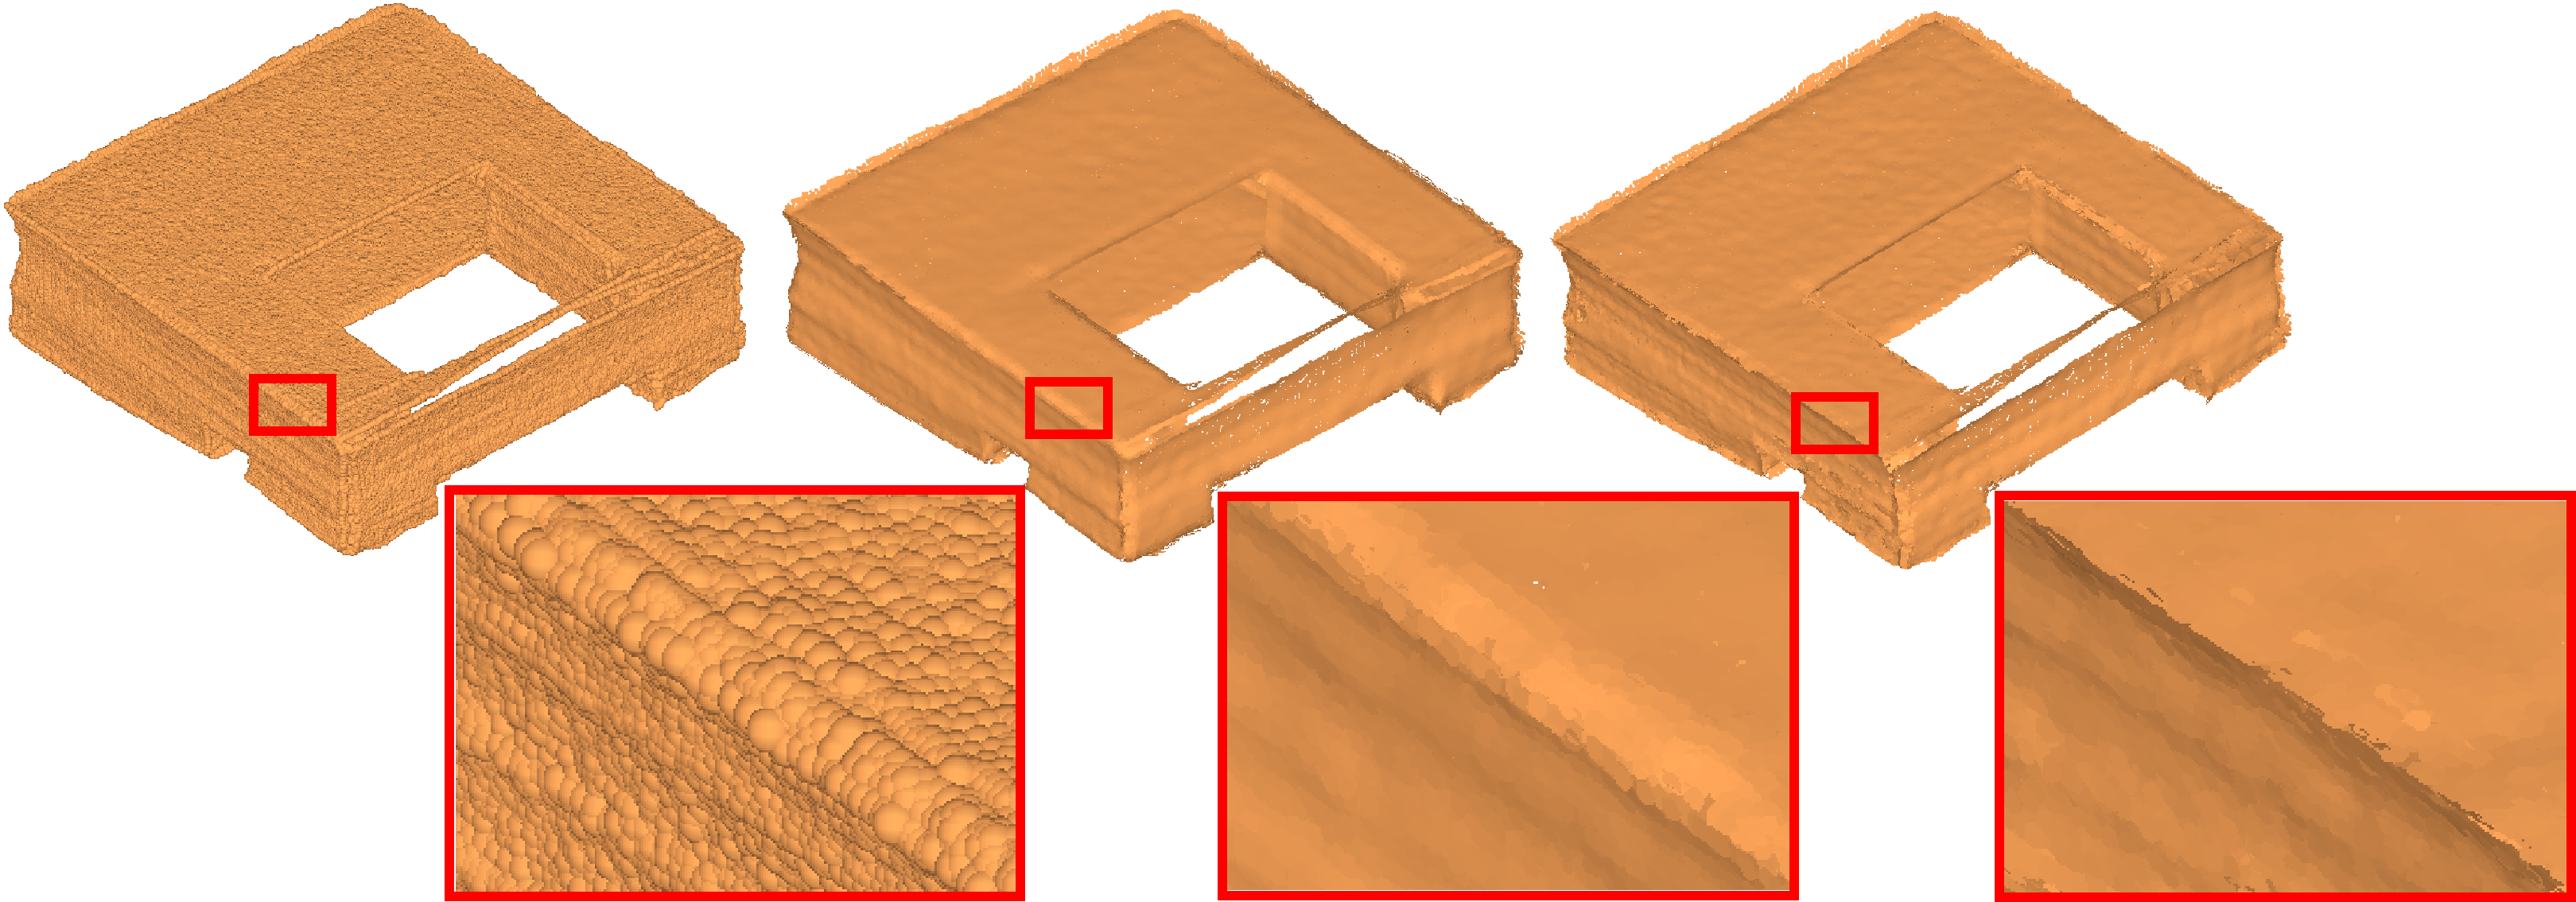
\includegraphics[width=1\linewidth]{box}
%    \end{tabular}
%    \caption{{\color{red}Normal estimation results for Box by using PCA and our algorithm. Left to
%     right are the raw scan, the results of PCA and our algorithm, respectively.}\label{fig:box}}
%\end{center}
\subsection{Implementation details}
\label{sec:implement}
%\textbf{Implementation details.}
The proposed approach has been implemented in Matlab and is not optimized for efficiency. All experiments have been performed with 1 CPU Intel(R) Xeon(R) 2.53GHz.
%
A typical example such as the Armadillon model with 99.4k points and 8.4k candidate feature points in~\fig~\ref{fig:realObjects}, takes a total of 4618 seconds. Of that time, candidate feature points selection, subneighborhood segmentation and normal estimation take 21, 4595 and 2 seconds respectively.
%-
As stated in section~\ref{sec:timing}, the most time-consuming operation is to solve~\eq~(\ref{eq:RSSLRR}) when segmenting subneighborhood of size $S^{*}$ for each candidate feature point.
A parallel C++ implementation with the linearized alternating direction approach \cite{LinLS11} could increase the performance remarkably.
